%----------
% Résultats
%----------

\chapter*{Résultats}
\addcontentsline{toc}{chapter}{Annexe 3 : Résultats}

Les programmes \textbf{hello\_world} et \textbf{thread} utilisés pour les
tests sont les suivants :

\begin{figure}[H]
	\begin{center}
		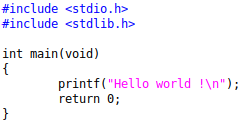
\includegraphics[scale=0.7, left]{\patchResults/hello_world_program}
	\end{center}
\end{figure}

\begin{figure}[H]
	\begin{center}
		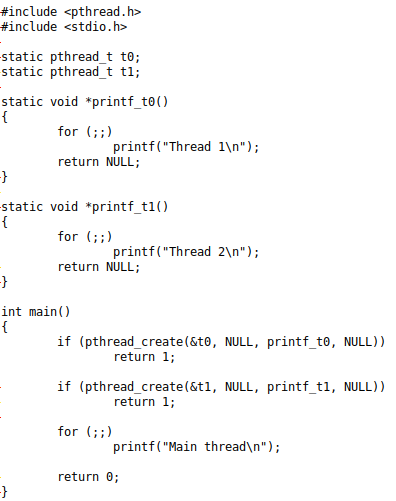
\includegraphics[scale=0.7, left]{\patchResults/thread_program}
	\end{center}
\end{figure}

%\newpage
%\section*{perf record -e cs\_etm/@tmc\_etf0/u --per-thread ./thread}
%Cet example montre le formatage dans la sortie standard suivant la commande
%\textbf{perf report --stdio}.

%\begin{figure}[H]
%        \begin{center}
%                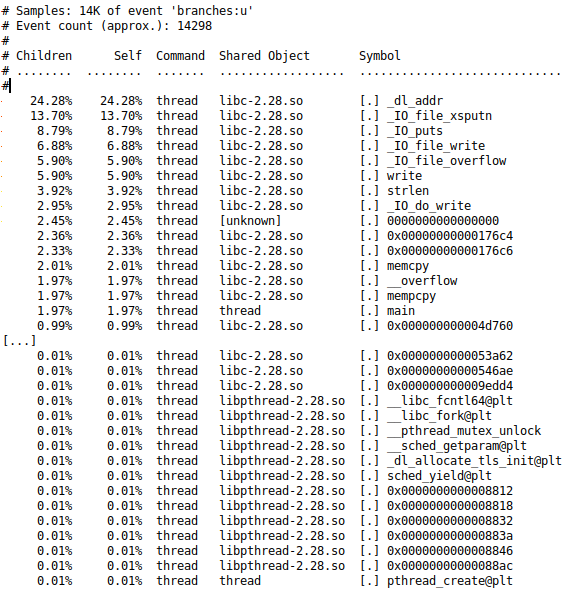
\includegraphics[width=\textwidth]{\patchResults/record_u_per_thread_thread}
%        \end{center}
%\end{figure}

%\newpage
%\section*{perf record -e cs\_etm/@tmc\_etf0/u --per-thread ./hello\_world}
%Cet example montre le formatage dans la sortie standard suivant la commande
%\textbf{perf report --stdio}.

%\begin{figure}[H]
%        \begin{center}
%                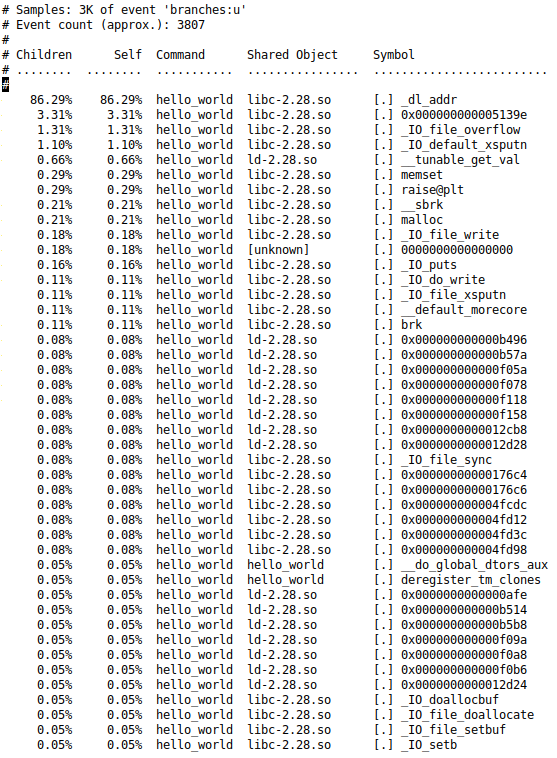
\includegraphics[width=\textwidth]{\patchResults/record_u_per_thread_hello_world}
%        \end{center}
%\end{figure}

%\newpage
%\section*{perf record -e cs\_etm/@tmc\_etf0,timestamp/k,branches --all-cpus ./hello\_world}
%Cet example montre le formatage dans la sortie standard suivant la commande
%\textbf{perf report --stdio}.

%\begin{figure}[H]
%        \begin{center}
%                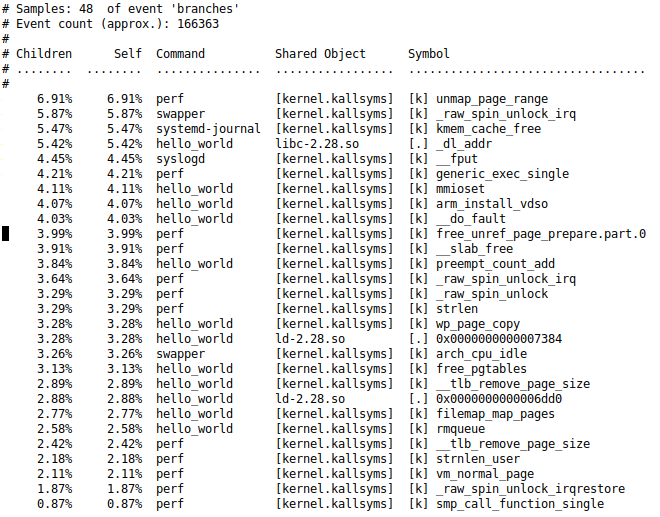
\includegraphics[width=\textwidth]{\patchResults/record_tmc_etf0_timestamp_k_branches_all_cpus_hello_world_0}
%        \end{center}
%\end{figure}

\newpage
\section*{perf record -vvv -e cs\_etm/contextid,freq,@tmc\_etf0/k,instructions --all-cpus ./hello\_world}
Cet example montre le formatage avec la librairie NCurses suivant la commande
\textbf{perf report}.

\begin{figure}[H]
	\begin{center}
		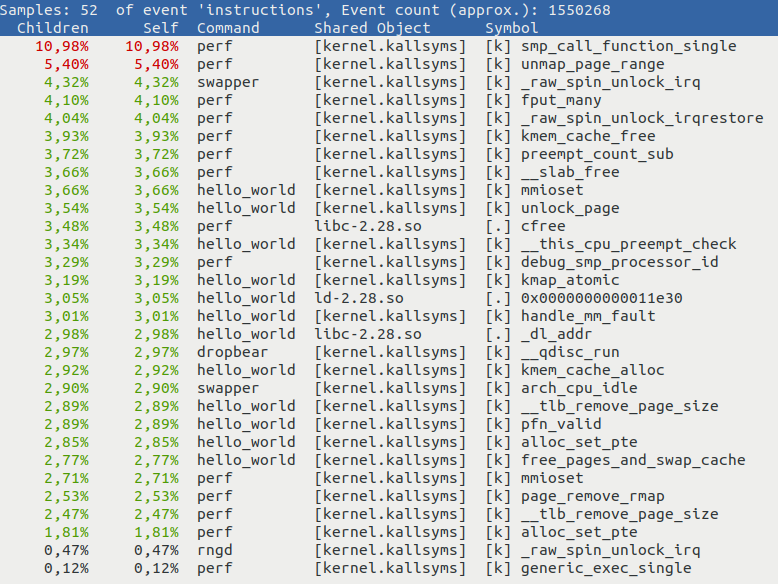
\includegraphics[width=\textwidth]{\patchResults/record_cs_etm_contextid_freq_@tmc_etf0_k_instructions_all_cpus_hello_world_0}
	\end{center}
\end{figure}

\begin{figure}[H]
	\begin{center}
		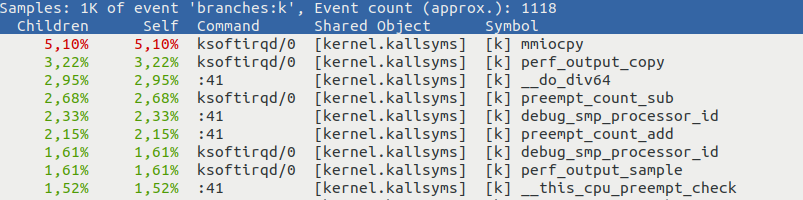
\includegraphics[width=\textwidth]{\patchResults/record_cs_etm_contextid_freq_@tmc_etf0_k_instructions_all_cpus_hello_world_1}
	\end{center}
\end{figure}

\begin{figure}[H]
	\begin{center}
		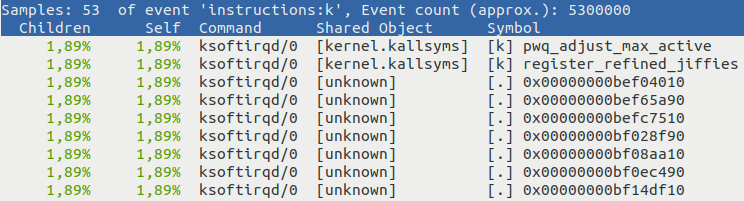
\includegraphics[width=\textwidth]{\patchResults/record_cs_etm_contextid_freq_@tmc_etf0_k_instructions_all_cpus_hello_world_2}
	\end{center}
\end{figure}



